\section{Konzept}\label{sec:konzept}
Anhand der Umfrage wurde ein Konzept für einen Sprachassistenten entwickelt. Dabei wurden die Kosten für benötigte Ressourcen vernachlässigt. Eine wichtige Anforderung an das Konzept ist der Datenschutz. Die Entwurfsprinzipien für die mehrseitige Sicherheit von Daten nach Kai Rannenberg stellt folgende vier Punkte in den Vordergrund \cite{kairannenberg}:

\begin{enumerate}
	\item Datensparsamkeit
	\item Kontrollmöglichkeiten für den Nutzer 
	\item Auswahlmöglichkeiten und Verhandlungsspielräume 
	\item Dezentralisierung und Verteilung
\end{enumerate} 

Im Rahmen dieses Konzepts erfolgt die Fokussierung auf die ersten drei Punkte. Oftmals erfassen Anwendungen Daten eines Nutzers, die nicht zur Verbesserung der Anwendungen sondern zur Analyse der Nutzer und dem Weiterverkauf verwendet werden. Deshalb soll durch das Konzept sichergestellt werden, dass eine Anwendung nur Daten von Nutzern bezieht, die diese auch tatsächlich benötigen. Des Weiteren sollen die erfassten Daten den Nutzern transparent dargestellt werden. Somit können Nutzer ihre erfassten Daten auch manipulieren bzw. anonymisieren. 

Daraus ergibt sich für den zu entwickelnden Sprachassistenten folgende Anforderungen:
\begin{itemize}
	\item User-Controlled-Privacy
	\item Funktionalität
	\item Performance
	\item Nutzerfreundlichkeit	
\end{itemize}

Durch User-Controlled Privacy kann ein Nutzer bestimmen, welche Daten er von sich für bestimmte Anwendungen freigibt. Anwendungen benötigen jedoch auch Daten eines Nutzers, um dadurch Nutzerfreundlichkeit zu bieten. Ein Beispiel ist die Frage eines Sprachassistenten nach der Wettervorhersage. Weiß der Sprachassistent wo sich ein Nutzer gerade befindet, so kann dieser die Wettervorhersage für die aktuelle Position des Nutzer liefern. Sonst müsste der Sprachassistent zuerst den Nutzer Fragen, für welchen Ort dieser eine Wettervorhersage geben soll. Will ein Nutzer seine Daten für eine Anwendung nicht freigeben, so kann er einen fiktiven Kontext festlegen. Damit kann der Nutzer die Anwendungen nutzen, jedoch auf Kosten der Nutzerfreundlichkeit.

Ein Kontext beschreibt die Eigenschaften eines Nutzers und ist sehr umfangreich, wie in Abbildung \ref{fig:kontext} zu sehen. Als Beispiele sind hierfür der kulturelle Hintergrund, die eigenen Interessen und Hobbys sowie das soziale Umfeld zu nennen.

\begin{figure}[!h]
	\centering
	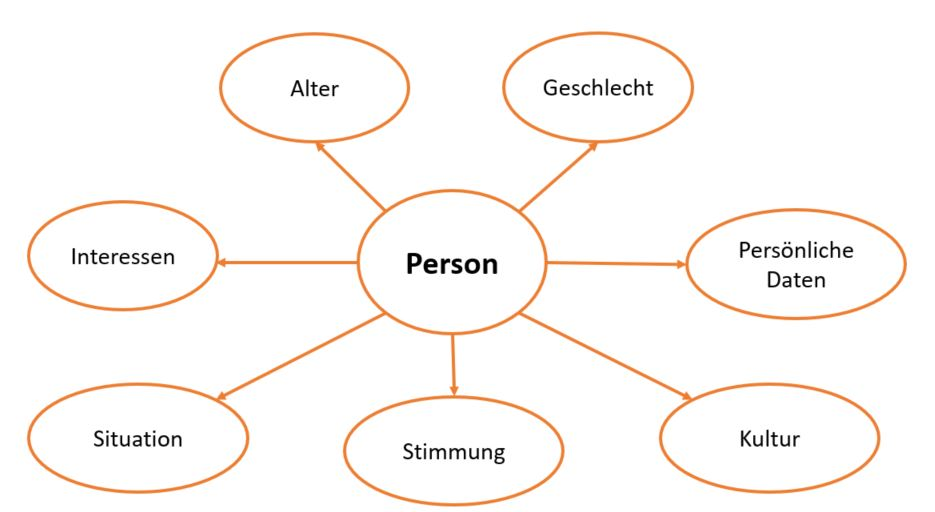
\includegraphics[width=1\linewidth]{Picture/Kontext}
	\caption[Nuzter Kontext]{Nuzter Kontext}
	\label{fig:kontext}
\end{figure}





